\documentclass{article}

\usepackage{enumitem}
\usepackage{graphicx}
\usepackage{listings}

\begin{document}

\title{CS 325: Project 1}
\author{Jared Wasinger}

\maketitle

\section{Enumeration}
  \subsection{Mathematical Analysis}
    \begin{verbatim}
maxSum = SMALLEST_NUMBER
for i = 0; i < list_length; i++:
  currentSum = 0

  for k = i; k < 
    \end{verbatim}

  \subsection{Experimental Analysis}
    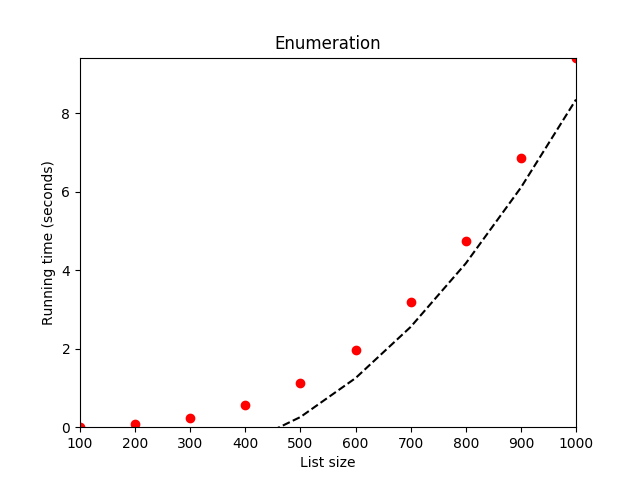
\includegraphics{enumeration.png}
    \textbf{Line of Best-fit:}\\
    $1.56639883*10^{-5}x^2 - 7.31257330*10^{-3}x + 8.2016835*10^{-1}$\\\\

    An equation of degree 2 was used to model the performance of this algorithm in order to capture the growth.  As expected, the enumeration algorithm performed the worst.  The relationship between input size and runtime was in accordance with $\Omega(n^3)$.\\

    \textbf{Predicted input size 10 seconds:} 12.30\\
    \textbf{Predicted input size 30 seconds:} 30\\
    \textbf{Predicted input size 60 seconds:} 73.7\\


\section{Better Enumeration}
  \subsection{Mathematical Analysis}
  \subsection{Experimental Analysis}
    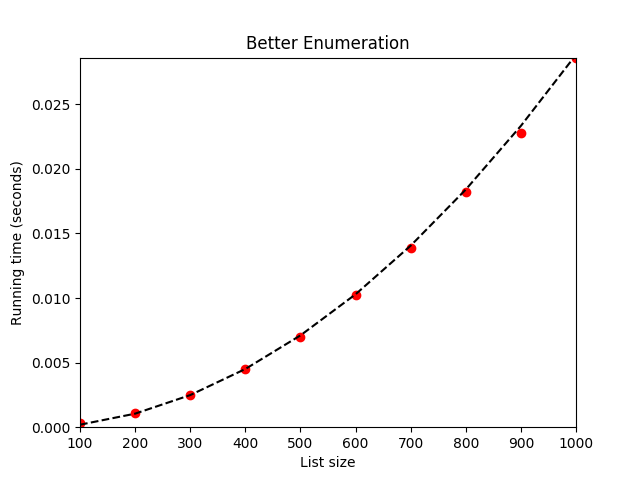
\includegraphics{better_enumeration.png}
    \textbf{Line of Best-fit:}\\
    $2.90793000*10^{-8}x^2 - 1.66918292e*10^7x - 8.17537308*10^5x$

    Like enumeration, the runtime of better enumeration grew exponentially as a function of input size.  However, the performance was dramatically improvemed compared from brute-force enumeration.\\

\section{Linear Time}
  \subsection{Mathematical Analysis}
  \subsection{Experimental Analysis}
    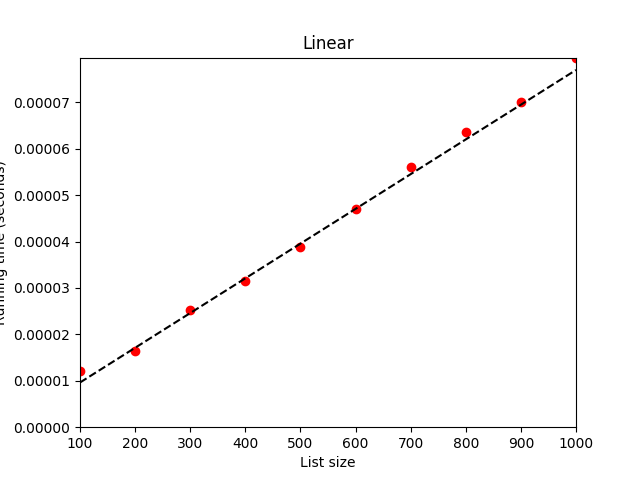
\includegraphics{linear.png}
    \textbf{Line of Best-fit:}\\
    $7.48200850*10^8x + 2.14576721*10^{-6}$

    As expected, the linear time algorithm had a runtime proportionate to the input size.  Thus, an equation of order 2 was used to create a best fit model.\\
\end{document}
